\chapter{Introduction}
\chaptermark{Introduction}
\label{chapter:introduction}
	
	\section{Forssea Robotics}

		\subsection{Présentation de l'entreprise}

			\forssea{} est une jeune entreprise innovante en matière de robotique sous-marine. Elle propose des solutions industrielles à l'exploration de ce milieu particulièrement hostile à l'homme. Ils excellent principalement dans quatre domaines : la robotique autonome, l'ingénierie des \textit{Remotely Operated Vehicles} (\gls{ROV}s), la vision sous-marine et l'intelligence artificielle. Cette expertise leur vaut de travailler aux côtés de nombreux partenaires, comme le groupe Total, Thales, iXblue, DeepOcean, et bien d'autres, mais aussi avec des centres de recherches comme l'\gls{ENSTAB}\footnote{\url{https://forssea-robotics.fr/index.php/about}}.

		\subsection{Présentation des produits}

			\forssea{} commercialise deux \gls{ROV}s\footnote{\url{https://forssea-robotics.fr/index.php/products/rovs}}, \argos{} et \atoll{}, visibles sur la \textsc{Figure}~\ref{fig:ROVs}. \argos{} est un robot d'intervention léger intelligent permettant d'embarquer une charge utile pesant jusqu'à $30\ kg$, tandis qu'\atoll{} est un robot de levage autonome qui peut porter jusqu'à $1500\ kg$. Il permet de déplacer et de positionner des structures sur les fonds marin, comme des balises \textit{Long Baseline} utilisées dans la localisation sous-marine~\cite{milne1983underwater}. Une structure portant une balise \textit{Long Baseline} est aussi visible sur la \textsc{Figure}~\ref{fig:ROVs}.

			\begin{figure}[!htb]
				\centering
				\begin{subfigure}[t]{0.3\textwidth}
					\centering
					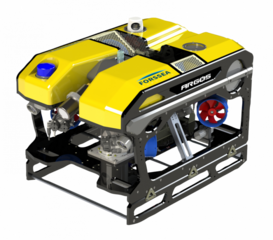
\includegraphics[width=\textwidth]{imgs/argos.png}
					\caption{\argos{}}
				\end{subfigure}
				\hfill
				\begin{subfigure}[t]{0.3\textwidth}
					\centering
					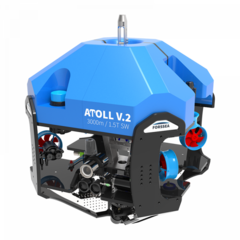
\includegraphics[width=\textwidth]{imgs/atoll.png}
					\caption{\atoll{}}
				\end{subfigure}
				\hfill
				\begin{subfigure}[t]{0.3\textwidth}
					\centering
					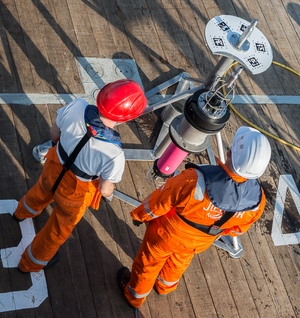
\includegraphics[width=\textwidth]{imgs/frame.png}
					\caption{Structure sous-marine et balise}
				\end{subfigure}
				\caption{\gls{ROV}s proposés par \forssea{} et structure sous-marine}
				\label{fig:ROVs}
			\end{figure}

			Ils proposent aussi plusieurs solutions de captations visuelles\footnote{\url{https://forssea-robotics.fr/index.php/products/cameras}}. Il y a la \textit{Navcam} qui est une caméra embarquant des algorithmes de traitement permettant de réaliser du positionnement visuel et l'\textit{Obscam} qui est une caméra d'observation.

	\section[Projet de fin d'études]{Présentation du projet de fin d'études}

		\subsection{Cadre professionnel}

			Ce projet de fin d'étude s'inscrit dans le cadre d'un contrat de professionnalisation réalisé chez Forssea Robotics, entre octobre 2020 et octobre 2021. Il m'a permis d'effectuer un premier pas dans le monde industriel tout en finissant ma formation à l'\gls{ENSTAB}. J'ai donc pu avoir à ma charge un sujet plus complet étant donnée la durée de ce stage, mais j'ai aussi pu avoir plus de responsabilités dans la gestion de ce projet, dans la mesure ou j'ai intégré l'équipe robotique de \forssea{} pendant une année complète dont six mois à temps plein.

		\subsection{Présentation du sujet}

			Dans les phases de développements de ses \gls{ROV}s, \forssea{} doit faire face à de nombreuses problématiques, dont celle de tester les algorithmes implémentés sur les \gls{ROV}s. Pour cela l'entreprise réalise régulièrement des tests et conditions réelles, mais ce sont des essais coûteux et qui prennent beaucoup de temps à planifier et à organiser. Afin de réduire le nombre d'essais nécessaires, il serait préférable de développer un moyen de test rapide et fiable des robots dans leur environnement. Cela permettrait d'améliorer les performances des robots tout en diminuant les coûts et les temps de développements.

		\subsection{Objectifs du projet}

			L'objectif de ce stage est donc de construire un environnement de simulation sous-marin pour \forssea{}. Il devra permettre de simuler au mieux le comportement des robots dans leur milieu, mais aussi être interfaçable avec le reste de l'implémentation logicielle pour tester leurs algorithmes de navigations autonomes. Cet environnement de simulation doit aussi permettre de tester les \gls{ROV}s dans des situations qui peuvent être difficiles à mettre en place lors d'expérimentations. Il est tout de même à noter qu'aucun simulateur ne saurait remplacer la réalisation de tests en conditions réelles.

	